\section{Data space estimators} 
\label{sec:ClosureEstimators}

In order to perform a quantitative analysis of the results obtained in the
closure tests, we discuss several estimators, which are computed from the
outcome of the closure test fits. These results depend on the pseudo-data that
have been generated and therefore are stochastic variables which can fluctuate.
The values of the estimators on a single replica will not tell anything about
the quality of our fits: we need to understand their probability distributions
in order to validate our fitting procedure. We begin this section by defining
estimators in data space, \ie\ estimators that are computed from the model
predictions for a set of experimental data points. Having defined the
estimators, we define criteria to characterise faithful uncertainties. We
conclude this section with a discussion of the predictions that can be obtained
for these estimators in the case of a linear model, where analytical
calculations can be performed. As we already saw in the previous section, the
analytical results cannot be applied directly to the NNPDF fits, but they are
useful examples that illustrate the expected behaviour of these quantities.

\subsection{Deriving the data space estimators}
\label{sec:ClosureEstimatorsDerivation}

For a given model $\modelvecrep$, obtained from fitting the $k$-th replica, we
start by defining the model error as the $\chi^2$ between the model predictions
and some data central values $\testset{\obspriorcent}$, normalised by the number
of data points
\begin{equation}
    \label{eq:chi2kereponerep}
    \frac{1}{\ndata} 
        \left( \testset{\fwdobsop}\left(\modelvecrep\right) - \testset{\obspriorcent} \right)^T
        \testset{\obspriorcov}^{-1}
        \left( \testset{\fwdobsop}\left(\modelvecrep\right) - \testset{\obspriorcent} \right)\, ,
\end{equation}
and we purposely denoted the data which the model error is evaluated on as
$\testset{\obspriorcent}$, as opposed to the training data $\obspriorcent$,
which is used to determine the model parameters. The corresponding covariance is
denoted $\testset{\obspriorcov}$. Note that in Eq.~\ref{eq:chi2kereponerep},
$\testset{\obspriorcent}$ is a stochastic variable, but also $\modelvecrep$ is a
stochastic variable, with its pattern of fluctuations, since the fitted model
depends on the data $\pseudodat^{\repind}$ that enter the fit. We define the
model error $\eout$ on the set of data $\testset{\obspriorcent}$ by taking the
average over the models,
\begin{align}
    \label{eq:chi2kerep}
    &\eout = \frac{1}{\ndata}\nonumber \\
    & \times \emodel{
        \left( \testset{\fwdobsop}\left(\modelvecrep\right) - \testset{\obspriorcent} \right)^T
        \testset{\obspriorcov}^{-1}
        \left( \testset{\fwdobsop}\left(\modelvecrep\right) - \testset{\obspriorcent} \right)
    }\, ,
\end{align}
where we defined the expectation value over the ensemble of model replicas as
\begin{equation}
    \emodel{x} \equiv \frac{1}{\nreps} \sum_{k=1}^{\nreps} x^{(k)} \, .
\end{equation}
We could of course set $\testset{\obspriorcent} = \obspriorcent$ and evaluate
the model performance on the fitted data however, as is common in machine
learning literature, we intend to use a separate set of test data. Ideally we
would choose $\testset{\obspriorcent}$ such that $\testset{\obspriorcent}$ and
$\obspriorcent$ are statistically independent, as in
Eq.~\ref{eq:JointIndepDataPrior}. This is achieved by choosing the split such
that the experimental covariance matrix is block diagonal:
\begin{equation}
    \modelpriorcov^{\rm total} =
    \begin{bmatrix}
        \modelpriorcov  & 0  \\ 
        0  & \testset{\modelpriorcov}  \\ 
    \end{bmatrix}\, .
\end{equation}

It is useful to perform a decomposition of Eq.~\ref{eq:chi2kerep}, following
usual manipulations of the likelihood function associated with least-squares
regression in~\cite{mlforphysics}. Least-squares regression is a special case of
minimum likelihood estimation, where the uncertainty on each data point is equal
in magnitude and uncorrelated. Here we review the decomposition in the more
general framework of data whose uncertainty is multigaussian. Starting with
Eq.~\ref{eq:chi2kerep} (evaluated on the ideal test data), we can complete the
square
\begin{align}
    \label{eq:EoutDecomposition}
        &\eout = \frac{1}{\ndata} \nonumber \\ 
        &\biggl\{ \emodel{
            \left( \testset{\fwdobsop}\left(\modelvecrep\right) - \testset{\law} \right)^T
            \testset{\obspriorcov}^{-1}
            \left( \testset{\fwdobsop}\left(\modelvecrep\right) - \testset{\law} \right)
        } + \nonumber\\
        &+ \emodel{
            \left( \testset{\law} - \testset{\obspriorcent} \right)^T
            \testset{\obspriorcov}^{-1}
            \left( \testset{\law} - \testset{\obspriorcent} \right)
        }+ \nonumber\\
        &+ 2 \emodel{
            \left( \testset{\fwdobsop}\left(\modelvecrep\right) - \testset{\law} \right)^T
            \testset{\obspriorcov}^{-1}
            \left(\testset{\law} - \testset{\obspriorcent} \right)
        }\biggr\}\, .
\end{align}
Let us now discuss these terms one by one, starting from the last two. The
second term is the shift associated with evaluating the model error on noisey
test data and the final term is a cross term which we will deal with later. We
therefore focus next on further decomposing the first term,
\begin{equation}
    \begin{split}
        &\emodel{
            \left( \testset{\fwdobsop}\left(\modelvecrep\right) - \testset{\law} \right)^T
            \testset{\obspriorcov}^{-1}
            \left( \testset{\fwdobsop}\left(\modelvecrep\right) - \testset{\law} \right)
        } = \\
        &= \mathbf{E}_{\{ \modelvec_* \}} \biggl[
            \left( \testset{\fwdobsop}\left(\modelvecrep\right) - 
            \emodel{\testset{\fwdobsop}\left(\modelvecrep\right)} \right)^T
            \testset{\obspriorcov}^{-1} \\
            &\quad\quad\times\left( \testset{\fwdobsop}\left(\modelvecrep\right) - 
            \emodel{\testset{\fwdobsop}\left(\modelvecrep\right)} \right)
         \biggr]+ \\
        &+ \left( \emodel{\testset{\fwdobsop}\left(\modelvecrep\right)} - \testset{\law} \right)^T
        \testset{\obspriorcov}^{-1}\\
        &\quad\quad\times\left( \emodel{\testset{\fwdobsop}\left(\modelvecrep\right)} - \testset{\law} \right)\, ,
    \end{split}
\end{equation}
where we have used the fact that the second term is constant across replicas and
the cross term that arises in this decomposition is zero when the expectation
value across replicas is taken. The first term in this expression we call the
{\em variance} and the second term is the {\em bias}.

As previously mentioned $\eout$ should be considered a stochastic estimator, in
theory we could take the expectation value across training data $\obspriorcent$
and test data $\testset{\obspriorcent}$. 
In other words, $\eout$ is a function of the Gaussian parameters $\eta$ and $\eta'$,
and we can take the average over them to compute the average over training and test data. 
Denoting as $\rho$ the Gaussian describing the distribution of $\eta$ and $\eta'$,
we can define
\begin{align}
    \mathbf{E}_{y}\left[\eout\right] = \int d\eta\, \rho\left(\eta\right) \eout\left(\eta\right)\,.
\end{align}
The average over the test data cancels the cross term in Eq.~\ref{eq:EoutDecomposition}
and the final result would be
\begin{equation}\label{eq:ExpectedBiasVariance}
    \mathbf{E}_{\obspriorcent} \mathbf{E}_{\testset{\obspriorcent}}[\eout] =
    \mathbf{E}_{\obspriorcent}[{\rm bias}] + 
    \mathbf{E}_{\obspriorcent}[{\rm variance}] +
    \mathbf{E}_{\testset{\obspriorcent}}[{\rm noise}]\,.
\end{equation}
We are not interested in the observational noise term, since it is independent
of the model and in the limit of infinite test data
$\mathbf{E}_{\testset{\obspriorcent}}[{\rm noise}] \to 1$. The two estimators of
interest are independent of the parameter $\eta'$ associated with the test data,
however they do depend implicitly of $\eta$, entering the definition of the training data used to determine
$\modelvecrep$.
Therefore we only need to take
the expectation value over the parameter $\eta$, associated with the training data. 
In practical terms, this can be
achieved by running multiple closure fits, each with a different observational
noise vector $\obsnoise$, and taking the average i.e.
\begin{equation}
    \label{eq:average_over_training_data}
    \mathbf{E}_{\obspriorcent}[ x ] = \frac{1}{\nfits} \sum_{j=1}^{\nfits} x.
\end{equation}
Clearly this is resource intensive, and requires us to perform many fits. In
NNPDF3.0 \cite{nnpdf30}, single replica proxy fits were used to perform a study
of the uncertainties. Here we have expanded the data-space estimators used in
the closure fits and also will be using multiple full replica fits to calculate
various expectation values - made possible by our next generation fitting code.

\subsection{Geometric Interpretation}

It is possible to interpret the relevant data space estimators geometrically, by
considering a coordinate system where each basis vector corresponds to an
eigenvector of the experimental covariance matrix normalised by the square root
of the corresponding eigenvalue. An example of this is given in
Fig.~\ref{fig:diagram2destimators}, where for simplicity we have considered a
system with just two data points, \ie\ a two-dimensional data space, with a
diagonal covariance. The origin of the coordinate system is the true value of
the observable. The observational noise in these coordinates corresponds to a
unit circle centred in the origin as shown in
Fig.~\ref{fig:diagram2destimators}. If the experimental covariance is faithful,
there is a 68\%  probability that the experimental value $y_0$ is within this
unit circle. Fig.~\ref{fig:diagram2destimators} shows one possible instance of
$y_0$. Repeating the entire fit procedure multiple times requires generating new
sets of experimental data $y_0$. The average over $y_0$ mentioned above, is
precisely the average over multiple fits, restarting the procedure each time
from a new instance of $y_0$.

For a given $y_0$ the replicas are generated as a set of points Gaussianly
distributed around it and therefore, in the limit of a large number of replicas,
68\% of them will fall within a unit circle centred in $y_0$. This is the dashed
circe in the figure. Clearly there is also a 68\% probability that the true
value (\ie\ the origin in our plot) is inside this second circle. The model
predictions, one for each replica, are then a set of points, whose mean is
$E_\epsilon[g]$. The mean squared radius of those points is what we call the
variance. The bias is the l2-norm of the vector between the origin and the mean
of the model predictions. 

A faithful representation of the errors requires that the true value, \ie\ the
origin of the coordinate system in our figure, has 68\% probability of being
within 1$\sigma$ from the central value of the fit, which is given by
$E_\epsilon[g]$. Looking at the figure again, the probability for the origin to
be inside the shaded circle must be 68\%. We will discuss faithful errors in
more detail in the next subsection.
%
\begin{figure}[h!]
    \centering
    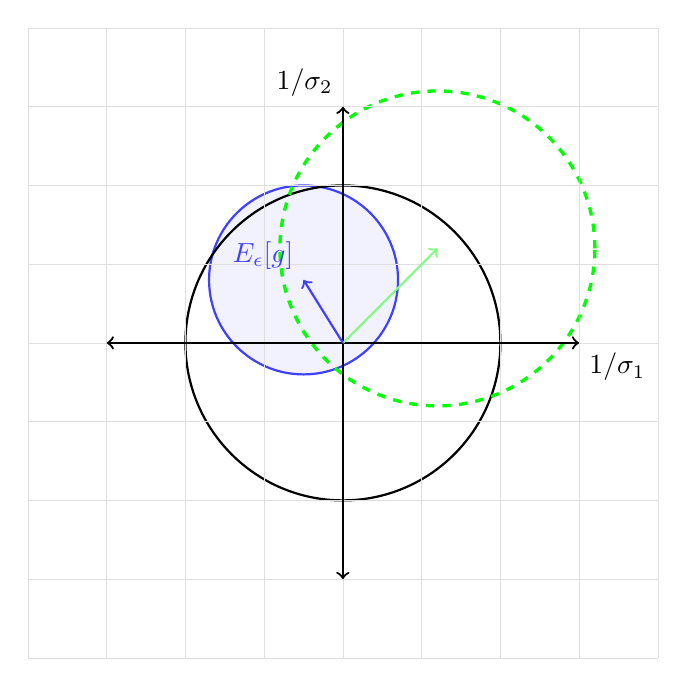
\begin{tikzpicture}
        \draw[blue!75, fill=blue!5, thick] (-0.5, 0.8) circle (1.2 cm);
        \draw[thick] (0,0) circle (2 cm);
        \draw[green, very thick, dashed] (1.2,1.2) circle (2 cm);
        \draw[step=1cm,gray!25!,very thin] (-4,-4) grid (4,4);
        \draw[thick,<->] (-3,0) -- (3,0) node[anchor=north west] {$1/\sigma_1$};
        \draw[thick,<->] (0,-3) -- (0,3) node[anchor=south east] {$1/\sigma_2$};
        \draw[green!50,thick,->] (0,0) -- (1.2,1.2) node[anchor=north west] {$\obspriorcent$};
        \draw[blue!75,thick,->] (0,0) -- (-0.5, 0.8) node[anchor=south east] {$E_\epsilon[g]$};
        \end{tikzpicture}
    \caption{Example of geometric interpretation of closure test estimators. The
    origin is the true observable values for each data point. The level one data
    (or experimental central values) are shifted away from this by $\obsnoise$.
    In this example the covariance matrix is diagonal, so the eigenvectors
    correspond to the two data points, the square root of the eigenvalues are
    simply the standard deviation of those points. This is without loss of
    generality because any multivariate distribution can be rotated into a basis
    which diagonalises the covariance matrix. The 1-sigma observational noise
    confidence interval is a unit circle centered on the origin. Some closure
    estimators can be understood as l2-norms of the vectors connecting points,
    i.e the bias is the l2-norm of the vector from the origin to the central
    value of the predictions.}
    \label{fig:diagram2destimators}
\end{figure}
%

\subsection{Faithful uncertainties in data space}

The two closure estimators of interest, bias and variance, can be used to
understand faithful uncertainties in a practical sense. If we return to
Eq.~\ref{eq:ExpectedBiasVariance} we can examine both estimators in a more
detail.

\paragraph{Variance}

The {\em variance} in the above decomposition refers to the variance of the
model predictions in units of the covariance
\begin{equation}
    \label{eq:VarDef}
    \begin{split}
        &\var = \frac{1}{\ndata}\mathbf{E}_{\{ \modelvec_* \}} \Big[ \\
            &\left( \testset{\fwdobsop}\left(\modelvecrep\right) - 
            \emodel{\testset{\fwdobsop}\left(\modelvecrep\right)} \right)^T
            \testset{\obspriorcov}^{-1}\\
            &\quad\quad\times\left( \testset{\fwdobsop}\left(\modelvecrep\right) - 
            \emodel{\testset{\fwdobsop}\left(\modelvecrep\right)} \right)
        \Big] \, ,
    \end{split}
\end{equation}
which can be interpreted as the model uncertainty in the space of the test data.
It is instructive to rephrase Eq.~\ref{eq:VarDef} as
\begin{equation}
    \label{eq:VarDefalternative}
    \var = \frac{1}{\ndata} {\rm Tr} \left[ \covrep \testset{\obspriorcov}^{-1} \right],
\end{equation}
where 
\begin{align}
    \label{eq:CovRep}
    \covrep = 
    &\mathbf{E}_{\{ \modelvec_* \}} \Big[
            \left( \testset{\fwdobsop}\left(\modelvecrep\right) - 
            \emodel{\testset{\fwdobsop}\left(\modelvecrep\right)} \right)\nonumber \\
            &\times\left( \testset{\fwdobsop}\left(\modelvecrep\right) - 
            \emodel{\testset{\fwdobsop}\left(\modelvecrep\right)} \right)^T
            \Big]
\end{align}
is the covariance matrix of the predictions from the model replicas. Note that
we can rotate to a basis where $\testset{\obspriorcov}$ is diagonal,
\begin{equation}
    \label{eq:InvCovPrimeDiag}
    \left(\testset{\obspriorcov}^{-1} \right)_{ij} = \frac{1}{\left(\testset{\sigma}_i\right)^2} 
    \delta_{ij}\, ,
\end{equation}
then we can rewrite Eq.~\ref{eq:VarDefalternative} as 
\begin{equation}
    \label{eq:VarianceInterpretation}
    \var = \frac{1}{\ndata}\, \sum_i \frac{\covrep_{ii}}{\left(\testset{\sigma}_i\right)^2}\, .
\end{equation}
The numerator in the right-hand side of the equation above is the variance of
the theoretical prediction obtained from the fitted replicas, while the
denominator is the experimental variance, the average is now taken over
eigenvectors of the experimental covariance matrix. Note that this ratio does
not need to be equal to one, the model error on a given point can be smaller
than the experimental one, since all theoretical estimates are correlated by the
underlying theoretical law. 

\paragraph{Bias}

Similarly, the {\em bias}\ is defined as the difference between the expectation
value of the model predictions and the true observable values in units of the
covariance, \ie 
\begin{align}
    \label{eq:BiasDef}
    \bias &= \frac{1}{\ndata}
    \left( \emodel{\testset{\fwdobsop}\left(\modelvecrep\right)} - \testset{\law} \right)^T
    \testset{\obspriorcov}^{-1} \nonumber\\
    &\times\left( \emodel{\testset{\fwdobsop}\left(\modelvecrep\right)} - \testset{\law} \right)\, .
\end{align}
The smaller the bias, the closer the central value of the predictions is to the
underlying law. In Eq.~\ref{eq:ExpectedBiasVariance}, the expectation value is
taken across the prior distribution of the training data, which yields
\begin{equation}
    \mathbf{E}_{\obspriorcent}[{\rm bias}] = \frac{1}{\ndata}
    {\rm Tr} \left[ \covcent \testset{\obspriorcov}^{-1} \right]\, ,
\end{equation}
where we have introduced $\covcent$ as the covariance of the expectation value
of the model predictions,
\begin{align}
    \label{eq:CovCentDef}
    \covcent &= 
    \mathbf{E}_{\obspriorcent}\Big[
        \left( \emodel{\testset{\fwdobsop}\left(\modelvecrep\right)} - \testset{\law} \right) \nonumber \\
        &\times\left( \emodel{\testset{\fwdobsop}\left(\modelvecrep\right)} - \testset{\law} \right)^T   
    \Big]\, .
\end{align}
The point is that the bias on the test data is a stochastic variable which
depends on the central value of the training data through $\modelvecrep$. The
matrix $\covcent$ describes the fluctuations of the central value of the model
prediction around the true observable values as we scan different realisations
of the training data. 

It is important to stress the difference between variance and bias. In the case
of the variance, we are looking at the fluctuations of the replicas around their
central value for fixed $\obspriorcent$. This is related to the ensemble of
model replicas we provide as the end product of a fit and can be calculated when
we have one instance of $\obspriorcent$, provided by the experiments. In the
case of the bias we consider the fluctuations of the central value over replicas
around the true theoretical prediction as the values of $\obspriorcent$
fluctuate around $\law$. This latter procedure is only possible in a closure
test, where the underlying true observable is known. The bias as defined here
yields an estimate of the fluctuations of the MAP estimator if we could do
multiple independent instances of their measurements from each experiment.

\paragraph{Bias-variance ratio}

Finally, the {\em bias-variance ratio} is defined as
\begin{equation}
    \label{eq:RatioDef}
    \biasvarratio \equiv \sqrt{\frac{
        \mathbf{E}_{\obspriorcent}[ \bias ]}{
            \mathbf{E}_{\obspriorcent}[ \var ]}}\, ,
\end{equation}
where we have taken the square root, since bias and variance are both mean
squared quantities. The value of $\biasvarratio$ yields a measurement of how
much uncertainties are over or under estimated. If the uncertainties are
completely faithful, then $\biasvarratio = 1$. We note that $\biasvarratio$ is
not completely general: it is not a measure defined in model space and depends
on the choice of test data. Therefore it only gives {\em local} information on
the model uncertainties. If the distribution of the expectation value of model
predictions is gaussian centered on the true observable values, with covariance
$\covcent$ and the distribution of the model replicas is also gaussian, with
covariance $\covrep$ then model uncertainties are faithful if
\begin{equation}\label{eq:IdealRatioDef}
    \covcent {\covrep}^{-1} = 1.
\end{equation}
The difficulty with calculating Eq.~\ref{eq:IdealRatioDef} comes from the fact
that $\covrep$ is likely to have large correlations which would lead it to be
singular or ill-conditioned. As a result, any error estimating $\covrep$ from
finite number of replicas could lead to unstable results. $\biasvarratio$
overcomes this instability by taking the ratio of the average across test data
of these matrices, in units of the experimental covariance matrix. There may
still be large relative errors for smaller eigenvalues of $\covrep$, but these
should not lead to instabilities in $\biasvarratio$ unless they correspond to
directions with very low experimental uncertainty. As an extra precaution, we
shall estimate an uncertainty on $\biasvarratio$ by performing a bootstrap
sample on fits and replicas.

\paragraph{Quantile statistics}
\label{sec:QuantileStatistics}

When the closure test was first presented in \cite{nnpdf30}, there was an
estimator introduced in the space of PDFs which also aimed to estimate
faithfulness of PDF uncertainties using the combined assumption of Gaussian PDF
uncertainties and quantile statistics, called $\xi_{1\sigma}$. Here we can
define an analogous expression in the space of data,
\begin{align}
    \label{eq:XiDataDef}
    &\xisigdat{n} = 
        \frac{1}{\ndata} \sum_{i}^{\ndata} \nonumber\\
        &\times\frac{1}{\nfits} \sum_{l}^{\nfits}
            I_{[-n \testset{\sigma}_i^{(l)}, n \testset{\sigma}_i^{(l)}]}
            \left( \emodel{\testset{\fwdobsop}_i}^{(l)} - \testset{\law}_i \right),
\end{align}
where $\testset{\sigma}_i^{(l)} = \sqrt{\covrep_{ii}}$ is the standard deviation
of the theory predictions estimated from the replicas of fit $l$ and $I_{[a,
b]}(x)$ is the indicator function, which is one when $a \leq x \leq b$ and zero
otherwise. In other words, $\xisigdat{n}$ is counting how often the difference
between the prediction from the MAP estimator and the true observable value is
within the $n\sigma$-confidence interval of the replicas, assuming they're
Gaussian. Since $\covrep$ is primarily driven by the replica fluctuations, we
assume that it is roughly constant across fits, or independent upon the specific
instance of observational noise. This allows us to write $\xisigdat{n}$ for a
specific data point in the limit of infinite fits, each to a different instance
of the data as
%
\begin{equation}
    \label{eq:XiIExpecVel}
        \xisigdati{n} =
            \int_{-\infty}^{\infty} I_{[-n \testset{\sigma}_i, n \testset{\sigma}_i]}\,
            \left( \emodel{\testset{\fwdobsop}_i}^{(l)} - \testset{\law}_i \right) 
            \rho(\obsnoise) \, 
            {\rm d}(\obsnoise) \, ,
\end{equation}
%
where $\emodel{\fwdobsop_i}^{(l)}$ has implicit conditional dependence on
$\obsnoise$. 
If the distribution of 
$$\emodel{\testset{\fwdobsop}_i}^{(l)} - \testset{\law}_i$$ is Gaussian, centered
on zero, we can define ${\testset{ \hat{\sigma} }}_i = \sqrt{\covcent_{ii}}$. In
this case
\begin{equation}
    \label{eq:expectedxi}
    \xisigdati{n} =
    \erf \left( \frac{n \testset{\sigma}_i}{\testset{\modelstd}_i \sqrt{2}}\right),
\end{equation}
which is simply the standard result of integrating a gaussian over some finite
symmetric interval.

The analogy between $\biasvarratio$ and $\xisigdat{n}$ is clear, the ratios of
uncertainties are both attempts to quantify Eq.~\ref{eq:IdealRatioDef} whilst
keeping effects due to using finite statistics under control. Whilst with
$\biasvarratio$ we take the average over test data before taking the ratio,
$\xisigdat{n}$ instead takes the ratio of the diagonal elements - ignoring
correlations. Since the predictions from the model will be compared with
experimental central values, taking into account experimental error, we find it
more natural to calculate $\xisigdat{n}$ in the basis which diagonalises the
experimental covariance of the test data as in Eq.~\ref{eq:InvCovPrimeDiag}. If
we assume that in this new basis, that both
$\frac{\covrep_{ii}}{\left(\sigma'_i\right)^2}$ and
$\frac{\covcent_{ii}}{\left(\sigma'_i\right)^2}$ are approximately constant for
all eigenvectors of the experimental covariance matrix, then we recover the
approximation
\begin{equation}\label{eq:CompareXiRatio}
    \xisigdat{n} \sim \erf \left( \frac{ n\biasvarratio}{\sqrt{2}} \right).
\end{equation}
Whilst it is clear that Eq.~\ref{eq:CompareXiRatio} is reliant on a fair few
assumptions which may not hold, we will use the comparison of $\xisigdat{n}$ with
$\biasvarratio$ to consider how valid these assumptions may be.

\subsection{Closure estimators - Linear problems}
\label{Sec:LinearMapEstimators}

Once again we return to the linear model framework set out in
Sec.~\ref{sec:fluct-fit-values}. We can perform an analytical closure test in
this framework, and check our understanding of the closure estimators. Consider
the true observable values for the test data are given by
\begin{equation}
    \label{eq:LinearLawMap}
    \testset{\law} = \testset{\fwdobsop} \lawmodel
\end{equation}
where $\lawmodel \in \modelspace$, and we assume that the number of (non-zero)
parameters in the underlying law is less than or equal to the number of
parameters in the model, $\nlaw \leq \nmodel$. Using the previous results from
Sec.~\ref{sec:fluct-fit-values}, we can write down the difference between the
true observables and the predictions from the MAP estimator (or the expectation
of the model predictions across model replicas - in the linear model these are
the same)
\begin{equation}
    \begin{split}
        \emodel{\testset{\fwdobsop}\left(\modelvecrep\right)} - \testset{\law} &=
        \testset{\linmap} (\modelpostcent - \lawmodel ) \\
        &= \testset{\linmap} \modelpostcov \linmap^T \obspriorcov^{-1} \, \obsnoise \, ,
    \end{split}
\end{equation}
where we recall that $\linmap$ is the forward map to the training observables
and $\obspriorcent$ are the corresponding training central values. Because the
training observables do not necessarily coincide with the data used to compute
the estimators, we have two different maps $\linmap$ and $\linmap'$. Calculating
the covariance across training data of
$\emodel{\testset{\fwdobsop}\left(\modelvecrep\right)} - \testset{\law}$ gives
\begin{equation}
    \covcent = \testset{\linmap} \modelpostcov \testset{\linmap}^T \, ,
\end{equation}
so the full expression for $\mathbf{E}_{\obspriorcent}[{\rm bias}]$ is given by
\begin{equation}\label{eq:BiasLinearModel}
    \mathbf{E}_{\obspriorcent}[{\rm bias}] = \frac{1}{\ndata}
    {\rm Tr} \left[
        \testset{\linmap} \modelpostcov \testset{\linmap}^T
        \testset{\obspriorcov}^{-1}
    \right].
\end{equation}
We note that if the test data is identical the data the model was fitted on, we
recover an intuitive result $\mathbf{E}_{\obspriorcent}[{\rm bias}] =
\frac{\nmodel}{\ndata}$. In the case of a polynomial model, where the parameter
of the model are the coefficients of the polynomial function, the maximum value
which $\nmodel$ can take whilst $\linmap$ still has linearly independent rows is
$\ndata$ and in this case the $\mathbf{E}_{\obspriorcent}[{\rm bias}]$ takes its
maximum value of 1. The central predictions from the model exactly pass through
each data point.

We can perform a similar exercise on the model replica predictions. The
difference between the predictions from model replica $\repind$ and the
expectation value of the model predictions is
\begin{equation}
    \begin{split}
        \testset{\fwdobsop}\left(\modelvecrep\right) -
        \emodel{\testset{\fwdobsop}\left(\modelvecrep\right)} &=
        \testset{\linmap} (\modelvecrep - \modelpostcent) \\
        &= \testset{\linmap} \modelpostcov \linmap^T \obspriorcov^{-1} \, \noise \, .
    \end{split}
\end{equation}
Since $\noise$ and $\obsnoise$ follow the same distribution, it is clear that
\begin{equation}
    \covrep = \covcent,
\end{equation}
which simply means that
\begin{equation}
    \var = \mathbf{E}_{\obspriorcent}[{\rm bias}].
\end{equation}
We recall that when the map is linear, the NNPDF MC methodology generates
replicas which are sampled from the posterior distribution of the model given
the data. We have shown here that provided the underlying law belongs to the
model space, the posterior distribution of the model predictions satisfy the
requirement that $\biasvarratio = 1$.

We note that due to the invariance of the trace under cyclic permutations, we
can rearrange Eq.~\ref{eq:BiasLinearModel} as
\begin{equation}
    \mathbf{E}_{\obspriorcent}[{\rm bias}] = \frac{1}{\ndata}
    {\rm Tr} \left[
        \modelpostcov
        \testset{\linmap}^T \testset{\obspriorcov}^{-1} \testset{\linmap}
    \right] \, ,
\end{equation}
where the term $\testset{\linmap}^T \testset{\obspriorcov}^{-1}
\testset{\linmap}$ can be understood as the covariance matrix of the posterior
distribution in model space given the test data, with zero prior knowledge of
the model, which we denote as $\modelpostcov'$:
\begin{equation}\label{eq:BiasTraceModelPost}
    \mathbf{E}_{\obspriorcent}[{\rm bias}] = \frac{1}{\ndata}
    {\rm Tr} \left[ \modelpostcov {\modelpostcov}^{ \prime -1} \right] \, ,
\end{equation}
where we emphasise that the covariance matrices $\modelpostcov$ and
$\testset{\modelpostcov}$ are obtained from completely independent Bayesian
inferences with no prior information on the model parameters, unlike in
Eq.~\ref{eq:ModelPostSequential} where a sequential marginalisation causes
$\testset{\modelpostcov}$ to depend on $\modelpostcov$.

Alternatively, if we perform a sequential marginalisation of the data, and use
the result in Eq.~\ref{eq:ModelPostSequential}, but then take
$\testset{\obspriorcov}^{-1} \to 0$, \ie\ there is no information on the
observables in the test set, then the covariance of the posterior model
distribution is 
\begin{equation}
    \modelpostcov^{-1} = \linmap^T \obspriorcov^{-1} \linmap \, ,
\end{equation}
which is identical to the posterior model distribution given just the training
data - as one would expect. Now we can express bias (or variance) as
\begin{equation}\label{eq:BiasTraceObsPost}
    \mathbf{E}_{\obspriorcent}[{\rm bias}] = \frac{1}{\ndata}
    {\rm Tr} \left[
        \testset{\obspostcov}
        \testset{\obspriorcov}^{-1}
    \right] \, ,
\end{equation}
where $\testset{\obspostcov}$ is the covariance of the posterior distribution of
$\testset{\obs}$ with no prior information on that data. This might seem
peculiar because in determining $\testset{\obspostcov}$ we took the limit
$\testset{\obspriorcov}^{-1} \to 0$, which encodes the fact that we had no prior
information on the unseen data, however in Eq.~\ref{eq:BiasTraceObsPost} we
require $\testset{\obspriorcov}^{-1}$ to be finite. We rationalise
Eq.~\ref{eq:BiasTraceObsPost} as a comparison between the posterior distribution
in the space of data of some unseen observables to an independently determined
prior from performing the relevant experiment which measures the same
observables. The two distributions can be compared when the independently
measured experimental data is published.


\paragraph{Underparameterised model}

Note that if we were to choose the number of model parameters such that $\nlaw >
\nmodel$, then the variance would be unaffected, since the underlying law
parameters cancel. However, the bias would now contain an extra term from the
extra parameters in the underlying law, schematically:
\begin{align}
        &(\emodel{\testset{\fwdobsop}\left(\modelvecrep\right)} - \testset{\law})_i = \nonumber \\
        &\sum_{1 \leq j \leq \nmodel} \testset{\linmap}_{ij} (\modelpostcent - \lawmodel)_j -
        \sum_{\nmodel < j \leq \nlaw} \testset{\linmap}_{ij} \lawmodel_j,
\end{align}
which would mean that $\biasvarratio \neq 1$. This demonstrates that requiring
$\biasvarratio = 1$ demands that the model space is suitably flexible, if the
underlying law is parameterised then this can be summarised as requiring
$\lawmodel \in \modelspace$. Note that in the underparameterised regime the
model replicas are still drawn from the posterior distribution, however because
$\lawmodel \notin \modelspace$ we have somehow invalidated the assumptions that
go into the relation between model predictions and the data-space prior.

Although $\biasvarratio$ was largely chosen on practical grounds, we see that it
is still a stringent test that our assumptions are correct and that the
distribution our model replicas are drawn from is meaningful, this is what we
mean when we say {\em faithful uncertainties}.

An unfortunate trade-off when using $\biasvarratio$ is that it cannot be used as
a diagnostic tool, and is instead used simply for validation. For example, if
$\biasvarratio > 1$, then we cannot know whether there was a problem with the
fitting methodology used to generate the model replicas or a deeper issue such
as an inflexible model.
